\chapter{PHÂN TÍCH HỆ THỐNG}
\section{Kiến trúc tổng thể}
Hệ thống chọn mô hình IoT Gateway. Node A đọc DHT20 và điều khiển driver quạt; node B chuyển tiếp ESP-NOW/USB và cung cấp web cục bộ. PC tổng hợp, lưu bền, suy luận và kết nối CoreIOT. Trên cloud, sensor được đại diện bằng child device \code{room-node-01}, qua gateway \code{smartroom-pc-gateway}.
\begin{figure}[H]\centering
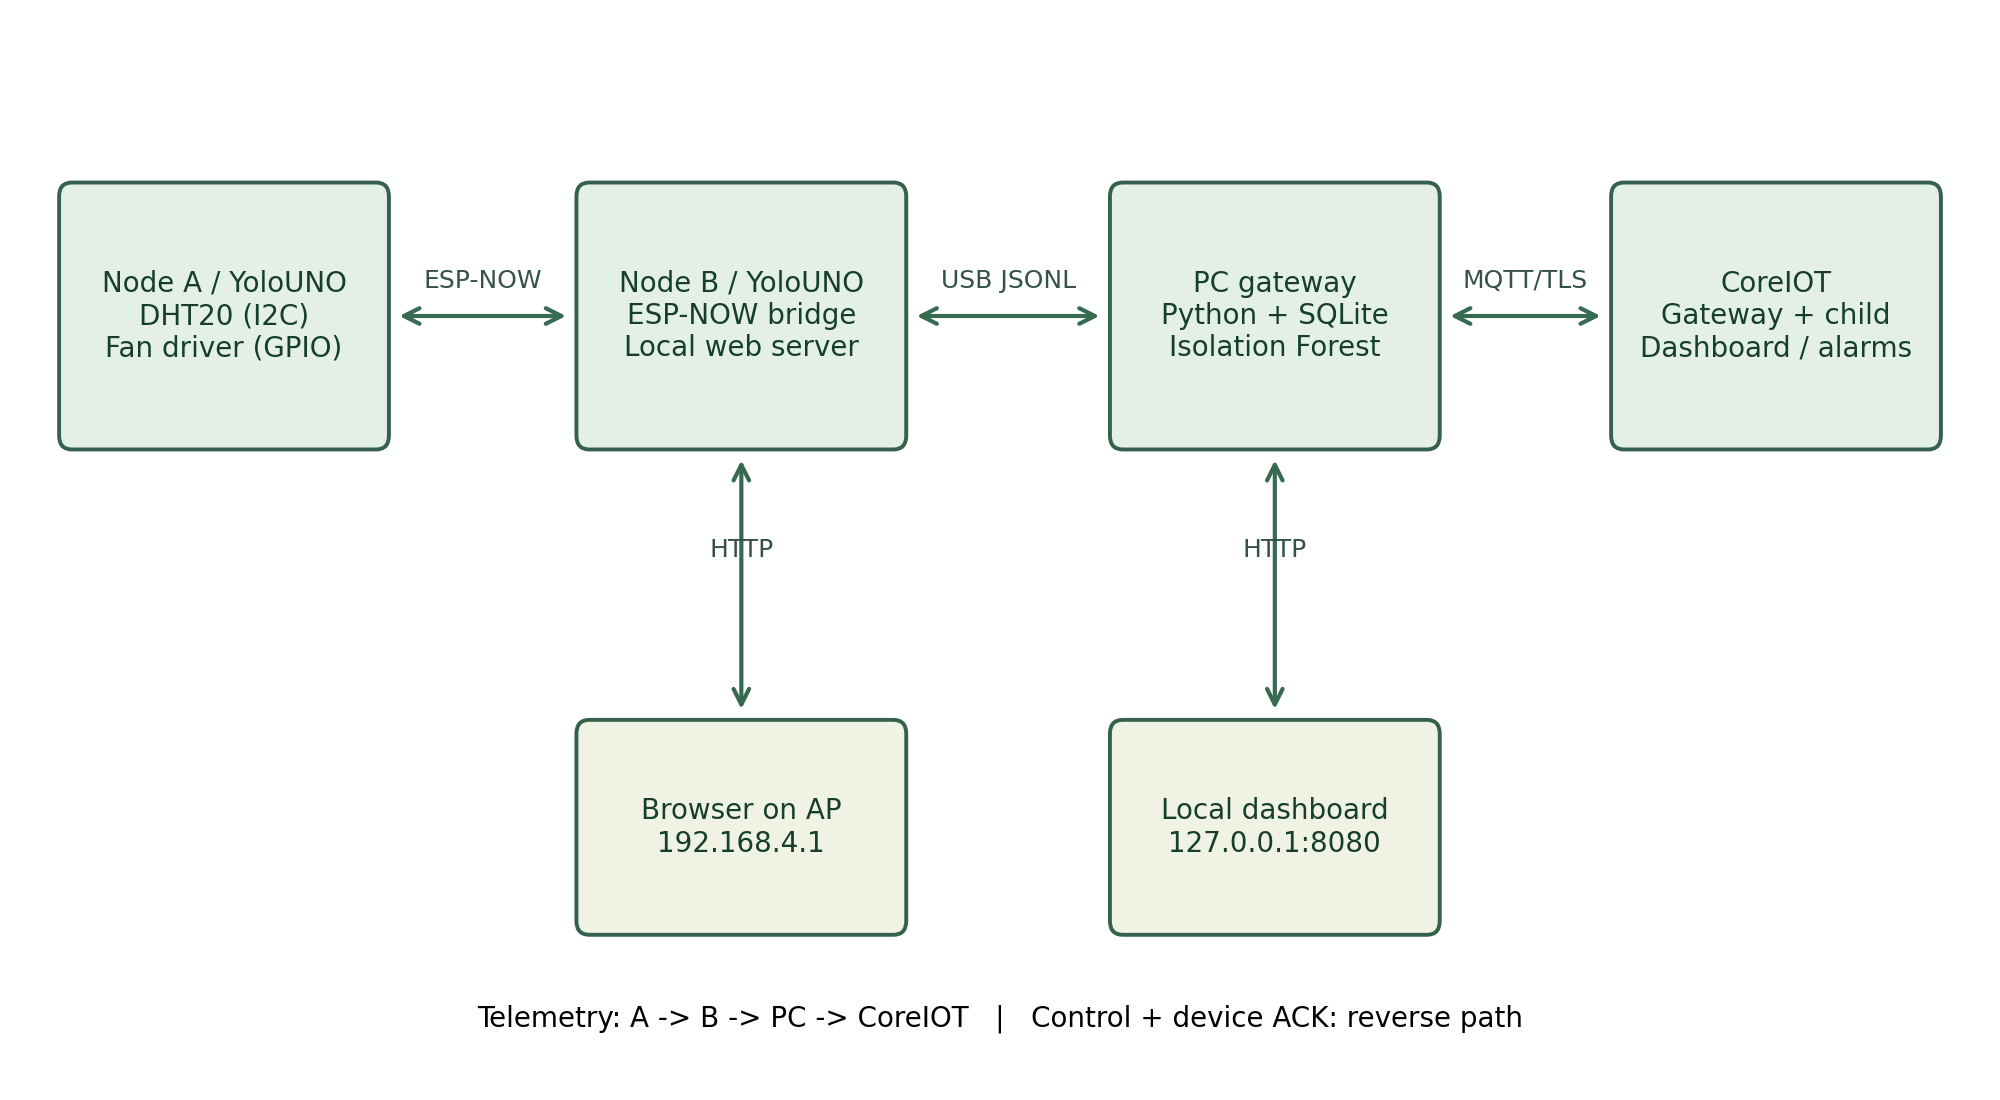
\includegraphics[width=\textwidth]{figures/architecture.png}
\caption{Kiến trúc thiết kế; mũi tên hai chiều thể hiện telemetry và điều khiển/ACK.}
\end{figure}
PC giúp cô lập phần kết nối cloud và AI khỏi firmware. USB Serial được chọn giữa bridge và PC để không bắt board vừa tham gia Wi-Fi Internet vừa đổi channel của ESP-NOW. PC có thể dùng Wi-Fi hoặc Ethernet riêng để ra Internet. Khi kiểm tra web bridge, người dùng có thể dùng điện thoại kết nối AP; nếu PC đổi sang AP bridge và mất Internet thì cloud tạm ngắt, outbox vẫn lưu dữ liệu.

\section{Phân rã chức năng}
Thu thập gồm đọc, kiểm tra mã lỗi, đóng gói, truyền và giải mã. Giám sát gồm kiểm tra cấu trúc, loại trùng, lưu đọc gần nhất và hiển thị. Phát hiện sự kiện gồm ngưỡng, hysteresis, AI và ghi journal. Điều khiển gồm kiểm tra tham số, cấp ID, retry, áp dụng GPIO, ACK và trả kết quả cho nguồn yêu cầu.
\begin{figure}[H]\centering
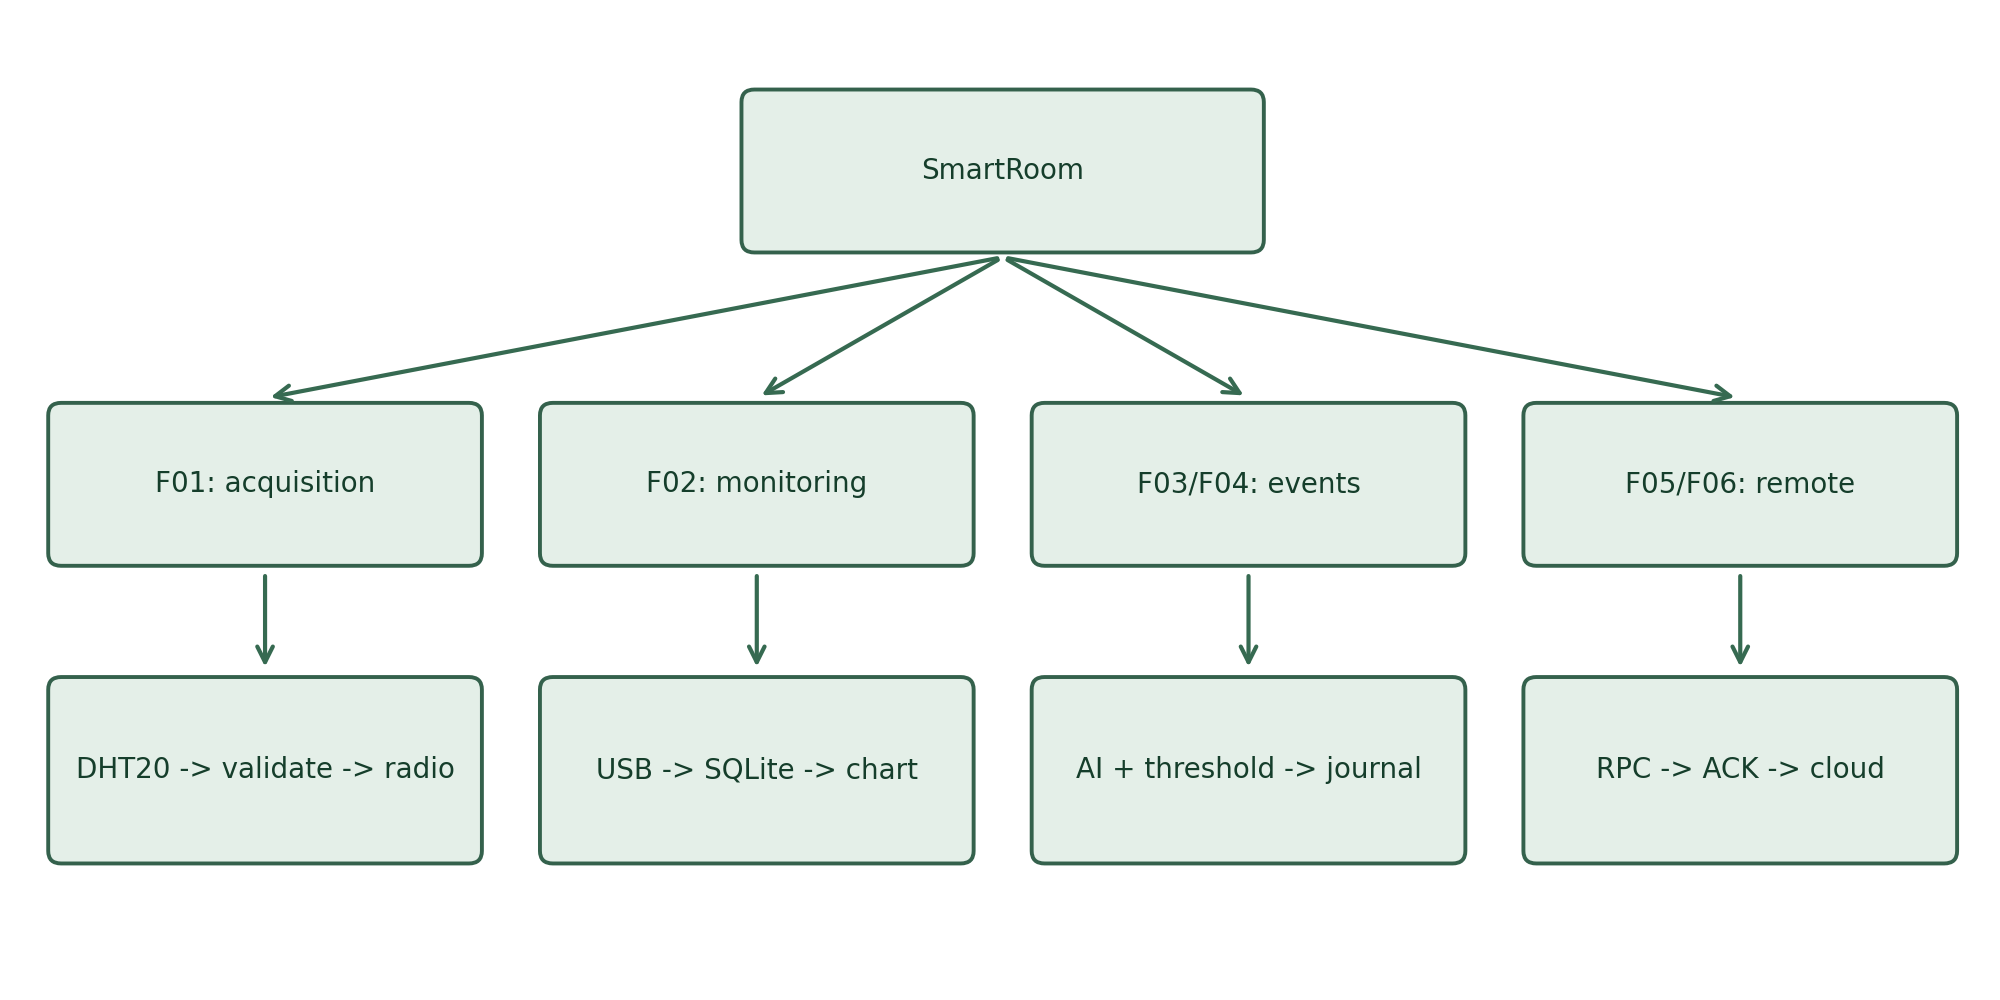
\includegraphics[width=\textwidth]{figures/decomposition.png}
\caption{Phân rã các chức năng chính của SmartRoom.}
\end{figure}

\section{Các lớp tính năng}
\subsection{Lớp cảm biến}
DHT20 được chọn vì có hai đại lượng trên cùng bus I2C và tài liệu kết nối YoloUNO \cite{ohstem}. Thư viện được ghim phiên bản và firmware kiểm tra kết quả \code{read()} trước khi truyền. Chu kỳ 2 giây phục vụ demo và không phải chế độ tối ưu năng lượng. Sai số thực nghiệm chưa đo với thiết bị tham chiếu; báo cáo không biến thông số nhà sản xuất thành sai số thực đã chứng minh.

T01 không được đăng ký vì đề bài yêu cầu cảm biến I2C \emph{trên Tasmota}. Việc sử dụng I2C trong Arduino không đáp ứng điều kiện đó. Đây là khác biệt cần nêu rõ khi ánh xạ tiêu chí.

\subsection{Lớp truyền thông}
ESP-NOW phục vụ liên kết node A--B, ánh xạ T06. Theo Espressif, peer cần được đăng ký và hai thiết bị phải ở channel thích hợp; khóa LMK bảo vệ unicast khi mã hóa được bật \cite{espnow}. Dự án cấu hình peer MAC tĩnh, channel 1 và key 16 byte phải thay khi triển khai. Khung riêng 25 byte nằm dưới giới hạn 250 byte của phiên bản ESP-NOW dùng trong build.

Gói có magic, version, type, boot, seq, command ID, nhiệt độ, độ ẩm và trạng thái fan. MAC nguồn được lọc; header và kích thước được kiểm tra. Telemetry không có retry ở tầng ứng dụng; mất gói cần đo bằng khoảng sequence theo từng boot. Lệnh được PC retry cùng ID để node không thực hiện lặp tác động.

USB dùng JSON một dòng một bản tin (JSONL). MQTT dùng QoS 1; token là của gateway. Mã hỗ trợ TLS với kiểm chứng CA hệ thống khi server cung cấp endpoint phù hợp. Với server lớp \code{app.coreiot.io}, profile riêng dùng cổng 1883 không TLS theo tài liệu chính thức \cite{coreiotconnect}. Paho cung cấp vòng lặp mạng và thông tin xác nhận publish \cite{paho}. Xác nhận broker không chứng minh cơ cấu vật lý đã chạy.

\subsection{Lớp IoT Gateway}
PC được chọn thay vì Raspberry Pi để tận dụng máy học tập sẵn có. Module xử lý không phụ thuộc Serial/MQTT nên có thể kiểm tra bằng clock và transport giả. SQLite lưu readings, events, commands và outbox. Một giao dịch lưu reading cùng bản tin chờ gửi tránh trường hợp có dữ liệu hiển thị nhưng không có bản tin để phát lại sau khởi động.

T08 bao gồm nhận dữ liệu và phân phối điều khiển hai chiều, không chỉ upload telemetry. T10 là HTTP dashboard tại loopback. T15 là tương tác với gateway/child trên CoreIOT: connect trước telemetry, re-register khi nối lại, nhận RPC có tên child và trả đúng request ID.

\subsection{Lớp trí tuệ nhân tạo}
Bài toán là phát hiện bất thường hai biến tại PC (T09). So với việc đưa TinyML lên board, hướng này dễ theo dõi dữ liệu, thay model và đo hiệu năng cho nhóm hai người. Isolation Forest được huấn luyện từ mẫu bình thường; \code{decision_function < 0} được xem là bất thường theo API thư viện \cite{isolation}.

Không dùng GPU và không đăng ký T04, T05 hoặc N04. Bộ dữ liệu mặc định được sinh có seed; dữ liệu thật có thể nhập CSV. Việc tách tập trước khi huấn luyện là yêu cầu phương pháp: không dùng nhãn/tập test để tạo hoặc điều chỉnh model. Kết quả từ dữ liệu sinh chỉ cho thấy pipeline hoạt động theo giả thiết sinh dữ liệu.

\subsection{Lớp ứng dụng và nền tảng CoreIOT}
Ứng dụng local do dự án viết hiển thị lịch sử, tuổi bản tin, AI, outbox và journal. N06 tập trung vào phát hiện và ghi sự kiện lâu dài; không tự nhận N05 chỉ vì giao diện co giãn trên điện thoại.

CoreIOT được chuẩn bị dashboard dựa trên template (T11), RuleChain (T12), hướng dẫn notification (T13) và adapter Gateway API (T15). Alarm và notification là hai chức năng khác nhau: alarm có bản ghi trạng thái; notification phải thực sự đến recipient. Rule engine cho phép nối các node xử lý theo quan hệ đầu ra \cite{ruleengine}.

\section{Ánh xạ tính năng -- yếu tố công nghệ}
\begin{table}[H]\centering\small
\caption{Ánh xạ tính năng với danh sách chấm điểm}
\begin{tabular}{P{1.1cm}P{5.8cm}P{3.3cm}P{4.3cm}}
\toprule Tính năng & Vai trò & Mã công nghệ & Khối thực hiện \\ \midrule
F01 & Cảm biến gửi dữ liệu không dây & T06 & Node A $\rightarrow$ B \\
F02 & Tổng hợp và giám sát local & T08, T10 & PC gateway \\
F03 & Phát hiện/ghi cảnh báo; xử lý cloud & T12, T13, N06 & PC và CoreIOT \\
F04 & Phân tích AI trên gateway & T09 & PC CPU \\
F05 & Điều khiển có ACK, web trên board & T07, T08, T10 & Hai board và PC \\
F06 & Telemetry/RPC theo child qua gateway & T08, T15 & PC và CoreIOT \\
F07 & Giao diện template và RuleChain & T11, T12, T13 & CoreIOT \\
F08 & Journal sự kiện và xuất CSV & T10, N06 & Dashboard/SQLite \\
\bottomrule
\end{tabular}
\end{table}
Các mã không chọn được liệt kê rõ trong bảng tự đánh giá ở đầu báo cáo. Cách chọn ưu tiên luồng demo thống nhất thay vì ghép nhiều giao thức không phục vụ vấn đề đã nêu.

\section{Công nghệ ngoài danh sách}
SQLite, HTTP/JSONL và thư viện Python là công cụ triển khai, không được cộng điểm công nghệ độc lập. SQLite cung cấp lưu trữ giao dịch và WAL, phù hợp outbox trên một máy tính \cite{sqlite}. HTTP giúp trình duyệt đọc trạng thái; JSONL giúp phân tách bản tin Serial có thể bị chia thành nhiều lần đọc. Joblib được dùng lưu model do dự án huấn luyện; chỉ nạp file tin cậy vì định dạng này có thể thực thi khi deserialize.

\section{Danh sách phần cứng}
\begin{table}[H]\centering\small
\caption{Cấu hình phần cứng dự kiến cần lấy tại lớp}
\begin{tabular}{c P{4.5cm}P{2.9cm}c P{5.6cm}}
\toprule STT & Thành phần & Giao tiếp & SL & Vai trò / điều kiện \\ \midrule
1 & YoloUNO ESP32-S3 & I2C/GPIO/ESP-NOW & 2 & Một sensor/actuator, một bridge; xác nhận revision/pinout. \\
2 & Module DHT20 & I2C & 1 & Đo nhiệt độ/độ ẩm; đối chiếu nguồn cấp và pull-up module. \\
3 & Quạt DC thấp áp và driver & GPIO vào driver & 1 bộ & Driver tương thích logic 3,3 V; không cấp tải từ GPIO. \\
4 & Cáp USB dữ liệu & USB CDC & 2 & Nạp và nối bridge; đóng monitor trước khi gateway mở cổng. \\
5 & Máy tính có Internet & USB + mạng & 1 & Python, SQLite, AI, MQTT/TLS và HTTP. \\
\bottomrule
\end{tabular}
\end{table}
Chưa chốt chi phí vì phần cứng dùng từ lớp và chưa xác nhận danh mục module thực tế. Dự án không yêu cầu mua thêm thiết bị chỉ để tăng số lượng mã chấm điểm.
